\chapter{Analisi descrittiva del dataset}
\label{cap:analisi_descrittiva}

% =============================================================================
\section{Panoramica Generale e Obiettivi dello Studio}
\label{sec:panoramica_dataset}
% =============================================================================

Il presente elaborato si propone di analizzare in modo rigoroso e multidisciplinare la relazione tra le abitudini di utilizzo dei social media --- con particolare riferimento alla piattaforma \textbf{Instagram} --- lo stile di vita quotidiano e gli indicatori di benessere psicofisico. Lo studio prende in esame un vasto patrimonio informativo composto originariamente da \textbf{$1.547.896$ profili utente} descritti attraverso \textbf{$58$ attributi} eterogenei (variabili numeriche continue, conteggi discreti, variabili categoriche nominali/ordinali e indicatori booleani).

L'architettura complessiva del documento è strutturata in tre fasi sequenziali e complementari:
\begin{enumerate}
    \item \textbf{Capitolo 1 --- Analisi Descrittiva del Dataset:} esamina la struttura globale dei dati ($N = 1.547.896$), cataloga le $58$ feature per dominio semantico, documenta il processo di \emph{Data Quality \& Cleaning} (confrontando la versione grezza \texttt{instagram\_usage\_lifestyle.csv} con la versione validata \texttt{instagram\_users\_lifestyle.csv}) e definisce il perimetro sperimentale focalizzato sulla popolazione dei \textbf{minorenni di età compresa tra $13$ e $17$ anni ($N = 146.258$)}.
    \item \textbf{Capitolo 2 --- Analisi di Classificazione (Apprendimento Supervisionato):} sviluppa e ottimizza modelli predittivi sulla coorte dei minorenni, affrontando il bilanciamento delle classi tramite tecniche combinate di \emph{oversampling} (\emph{SMOTE}) e \emph{undersampling} (\emph{ClusterCentroids}), la ricerca degli iperparametri ottimi (\emph{Grid Search}) e metodi di \emph{Ensemble Learning}.
    \item \textbf{Capitolo 3 --- Analisi di Clustering ed Esplorazione Approfondita (Apprendimento Non Supervisionato):} approfondisce l'Analisi Esplorativa dei Dati (\emph{EDA}) sulle metriche comportamentali e psicologiche dei minorenni, applica la selezione delle feature tramite studio della multicollinearità ($|r| > 0,80$), riduce la dimensionalità con una \textbf{PCA a distorsione zero ($k=5$ componenti)} e confronta tre algoritmi di clustering (\textbf{K-Means}, \textbf{DBSCAN} e \textbf{HDBSCAN}) per individuare i profili di rischio per la salute mentale (\emph{User Personas}) e gli \emph{Outlier} comportamentali.
\end{enumerate}

\begin{figure}[H]
    \centering
    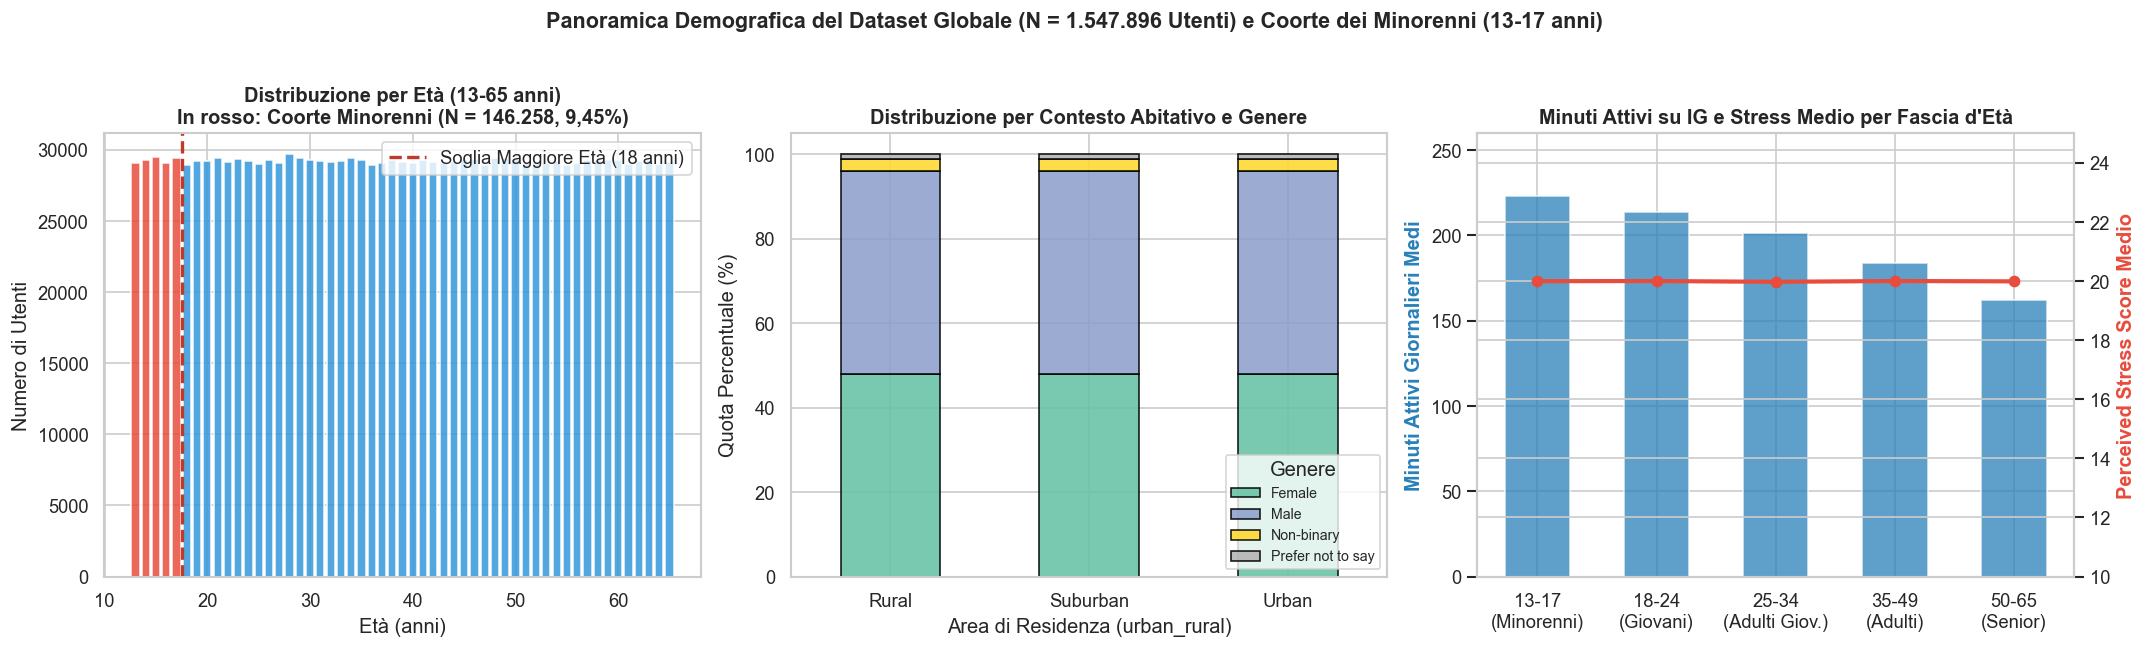
\includegraphics[width=\textwidth]{introduction/images/fig_desc01_demografia_globale.png}
    \caption{Panoramica demografica dell'intero dataset ($N = 1.547.896$ utenti, 13--65 anni): distribuzione per età con isolamento della coorte dei minorenni ($N = 146.258$, $9,45\%$), ripartizione per contesto abitativo e genere, e andamento del tempo attivo medio su Instagram e dello stress percepito per fascia d'età.}
    \label{fig:desc_demografia_globale}
\end{figure}

Come evidenziato nella Figura~\ref{fig:desc_demografia_globale}, la distribuzione per età copre uniformemente lo spettro compreso tra i $13$ e i $65$ anni (con una media globale di $38,99$ anni). Tuttavia, il pannello di destra rivela immediatamente il motivo scientifico per cui i capitoli di modellazione si concentrano sulla fascia \textbf{13--17 anni}: gli adolescenti minorenni registrano il \textbf{più alto tempo medio di esposizione giornaliera a Instagram ($223,21$ minuti/giorno, ovvero oltre $3\text{ ore e }43\text{ minuti}$)} abbinato al \textbf{più elevato punteggio medio di stress percepito ($19,99/40$)} rispetto a tutte le fasce d'età adulte.

% =============================================================================
\section{Catalogo Completo delle 58 Feature e Tipologia dei Dati}
\label{sec:catalogo_58_feature}
% =============================================================================

Il dataset originale presenta \textbf{$1.547.896$ righe e $58$ colonne}, senza alcun valore mancante (\texttt{NaN = 0} su tutte le colonne). Dal punto di vista della rappresentazione informatica, i $58$ attributi si suddividono in:
\begin{itemize}
    \item \textbf{31 variabili intere (\texttt{int64}):} identificativi, età, conteggi giornalieri/settimanali di interazioni (like, commenti, Reels, Stories, DM), minuti spesi nelle singole sezioni dell'app e punteggi psicologici discreti;
    \item \textbf{7 variabili reali in virgola mobile (\texttt{float64}):} ore lavorative settimanali, ore di sonno per notte, ore di esercizio fisico, indice di massa corporea (\texttt{body\_mass\_index}), durata media delle sessioni e punteggio composito di coinvolgimento (\texttt{user\_engagement\_score});
    \item \textbf{19 variabili testuali/categoriche (\texttt{object}):} attributi socio-demografici, abitudini alimentari e di stile di vita, preferenze sui contenuti e data di ultimo accesso (\texttt{last\_login\_date});
    \item \textbf{1 variabile booleana (\texttt{bool}):} indicatore di sottoscrizione a funzionalità premium (\texttt{uses\_premium\_features}).
\end{itemize}

Per facilitare la comprensione del dominio applicativo, le $58$ variabili sono state classificate in \textbf{7 macro-aree tematiche}, riportate integralmente nelle Tabelle~\ref{tab:cat_area123} e~\ref{tab:cat_area4567}.

\begin{table}[H]
\centering
\caption{Catalogo delle feature --- Parte I: Area Demografica e Socio-Economica (13 variabili), Salute Fisica e Stile di Vita (10 variabili), Benessere Psicologico (2 variabili).}
\label{tab:cat_area123}
\resizebox{\textwidth}{!}{%
\begin{tabular}{llp{4.2cm}p{6.8cm}}
\toprule
\textbf{Area Tematica} & \textbf{Nome Attributo} & \textbf{Tipo e Dominio / Range} & \textbf{Descrizione Semantica} \\
\midrule
\textbf{1. Demografia} & \texttt{user\_id} & \texttt{int64} ($1 \dots 1.547.896$) & Identificativo numerico univoco dell'utente (chiave primaria). \\
\textbf{e Contesto} & \texttt{age} & \texttt{int64} ($13 \dots 65$ anni) & Età anagrafica dell'utente (media globale: $38,99$ anni). \\
\textbf{Socio-Econ.} & \texttt{gender} & \texttt{object} (4 categorie) & Genere (\emph{Female} $48\%$, \emph{Male} $48\%$, \emph{Non-binary} $3\%$, \emph{Prefer not to say} $1\%$). \\
(13 feature) & \texttt{country} & \texttt{object} (10 categorie) & Paese di residenza (\emph{USA, India, Brazil, UK, Canada, Japan, Germany, Australia, South Korea, Other}). \\
 & \texttt{urban\_rural} & \texttt{object} (3 categorie) & Contesto abitativo (\emph{Urban} $55\%$, \emph{Suburban} $30\%$, \emph{Rural} $15\%$). \\
 & \texttt{income\_level} & \texttt{object} (5 classi ordinali) & Fascia di reddito (\emph{Low, Lower-middle, Middle, Upper-middle, High}). \\
 & \texttt{employment\_status} & \texttt{object} (6 categorie) & Stato occupazionale (\emph{Full-time, Student, Part-time, Self-employed, Unemployed, Retired}). \\
 & \texttt{education\_level} & \texttt{object} (6 classi ordinali) & Titolo di studio (\emph{High school, Bachelor's, Master's, Some college, Doctorate, Other}). \\
 & \texttt{relationship\_status} & \texttt{object} (5 categorie) & Stato civile/affettivo (\emph{Single, Married, In a relationship, Divorced, Widowed}). \\
 & \texttt{has\_children} & \texttt{object} (\emph{Yes / No}) & Presenza di figli a carico. \\
 & \texttt{weekly\_work\_hours} & \texttt{float64} ($0,0 \dots 80,0$ h) & Ore settimanali dedicate al lavoro retribuito. \\
 & \texttt{hobbies\_count} & \texttt{int64} ($0 \dots 10$) & Numero di hobby extracurriculari o passatempi praticati. \\
 & \texttt{social\_events\_per\_month} & \texttt{int64} ($0 \dots 15$) & Partecipazione mensile a eventi sociali dal vivo (offline). \\
\midrule
\textbf{2. Salute Fisica} & \texttt{sleep\_hours\_per\_night} & \texttt{float64} ($3,0 \dots 10,0$ h) & Ore medie di sonno per notte (media globale: $6,99$ h). \\
\textbf{e Abitudini} & \texttt{exercise\_hours\_per\_week} & \texttt{float64} ($0,0 \dots 20,0$ h) & Ore settimanali dedicate all'attività fisica o sportiva. \\
\textbf{Quotidiane} & \texttt{diet\_quality} & \texttt{object} (5 classi ordinali) & Qualità dell'alimentazione (\emph{Very poor, Poor, Average, Good, Excellent}). \\
(10 feature) & \texttt{smoking} & \texttt{object} (3 categorie) & Abitudine al fumo (\emph{Never, Former, Current}). \\
 & \texttt{alcohol\_frequency} & \texttt{object} (5 categorie) & Frequenza consumo alcolici (\emph{Never, Rarely, Weekly, Several times a week, Daily}). \\
 & \texttt{body\_mass\_index} & \texttt{float64} ($15,0 \dots 45,0$) & Indice di Massa Corporea (BMI). \\
 & \texttt{blood\_pressure\_systolic} & \texttt{int64} ($90 \dots 180$ mmHg) & Pressione arteriosa sistolica (massima). \\
 & \texttt{blood\_pressure\_diastolic} & \texttt{int64} ($60 \dots 120$ mmHg) & Pressione arteriosa diastolica (minima). \\
 & \texttt{daily\_steps\_count} & \texttt{int64} ($1.000 \dots 20.000$) & Conteggio medio giornaliero dei passi effettuati. \\
 & \texttt{books\_read\_per\_year} & \texttt{int64} ($0 \dots 30$) & Numero di libri letti in un anno. \\
\midrule
\textbf{3. Benessere} & \texttt{perceived\_stress\_score} & \texttt{int64} ($0 \dots 40$) & Punteggio clinico di stress percepito (scala PSS a 40 punti). \\
\textbf{Psicologico} & \texttt{self\_reported\_happiness} & \texttt{int64} ($1 \dots 10$) & Livello di felicità e soddisfazione vitale auto-dichiarata. \\
\bottomrule
\end{tabular}%
}
\end{table}

\begin{table}[H]
\centering
\caption{Catalogo delle feature --- Parte II: Volumi di Attività e Interazione su Instagram (13 variabili), Ripartizione del Tempo sull'App (7 variabili), Profilo Account, Preferenze e Metadati (13 variabili).}
\label{tab:cat_area4567}
\resizebox{\textwidth}{!}{%
\begin{tabular}{llp{4.2cm}p{6.8cm}}
\toprule
\textbf{Area Tematica} & \textbf{Nome Attributo} & \textbf{Tipo e Dominio / Range} & \textbf{Descrizione Semantica} \\
\midrule
\textbf{4. Volumi di} & \texttt{daily\_active\_minutes\_instagram} & \texttt{int64} ($5 \dots 590$ min/dì) & Tempo totale giornaliero trascorso attivamente su Instagram. \\
\textbf{Attività e} & \texttt{sessions\_per\_day} & \texttt{int64} ($1 \dots 50$ sessioni) & Numero di accessi giornalieri distinti all'applicazione. \\
\textbf{Interazioni IG} & \texttt{average\_session\_length\_minutes} & \texttt{float64} ($5,0 \dots 50,0$ min) & Durata media in minuti di ciascuna sessione di navigazione. \\
(13 feature) & \texttt{reels\_watched\_per\_day} & \texttt{int64} ($18 \dots 300$) & Numero di video brevi (\emph{Reels}) visualizzati al giorno. \\
 & \texttt{stories\_viewed\_per\_day} & \texttt{int64} ($10 \dots 150$) & Numero di \emph{Stories} visualizzate quotidianamente. \\
 & \texttt{likes\_given\_per\_day} & \texttt{int64} ($8 \dots 350$) & Numero di ``Mi piace'' assegnati ai contenuti ogni giorno. \\
 & \texttt{comments\_written\_per\_day} & \texttt{int64} ($0 \dots 80$) & Numero di commenti scritti giornalmente. \\
 & \texttt{posts\_created\_per\_week} & \texttt{int64} ($0 \dots 30$) & Numero di post pubblicati sul proprio profilo a settimana. \\
 & \texttt{dms\_sent\_per\_week} & \texttt{int64} ($0 \dots 97$) & Messaggi diretti (\emph{DM}) inviati settimanalmente. \\
 & \texttt{dms\_received\_per\_week} & \texttt{int64} ($0 \dots 111$) & Messaggi diretti (\emph{DM}) ricevuti settimanalmente. \\
 & \texttt{ads\_viewed\_per\_day} & \texttt{int64} ($0 \dots 62$) & Annunci pubblicitari sponsorizzati visualizzati al giorno. \\
 & \texttt{ads\_clicked\_per\_day} & \texttt{int64} ($0 \dots 20$) & Click effettuati sugli annunci pubblicitari giornalieri. \\
 & \texttt{user\_engagement\_score} & \texttt{float64} ($0,67 \dots 15,80$) & Indice sintetico di qualità e intensità dell'engagement. \\
\midrule
\textbf{5. Ripartizione} & \texttt{time\_on\_feed\_per\_day} & \texttt{int64} ($2 \dots 328$ min) & Minuti giornalieri trascorsi scorrendo il \emph{Feed} principale. \\
\textbf{del Tempo e} & \texttt{time\_on\_explore\_per\_day} & \texttt{int64} ($1 \dots 171$ min) & Minuti giornalieri trascorsi nella sezione \emph{Esplora}. \\
\textbf{Abitudini} & \texttt{time\_on\_messages\_per\_day} & \texttt{int64} ($1 \dots 138$ min) & Minuti giornalieri dedicati alla messaggistica diretta (\emph{DM}). \\
\textbf{Connesse} & \texttt{time\_on\_reels\_per\_day} & \texttt{int64} ($2 \dots 227$ min) & Minuti giornalieri dedicati alla visione di \emph{Reels}. \\
(7 feature) & \texttt{notification\_response\_rate} & \texttt{float64} ($0,0 \dots 1,0$) & Tasso di risposta immediata alle notifiche push ricevute. \\
 & \texttt{volunteer\_hours\_per\_month} & \texttt{float64} ($0,0 \dots 30,0$ h) & Ore mensili dedicate ad attività di volontariato. \\
 & \texttt{travel\_frequency\_per\_year} & \texttt{int64} ($0 \dots 15$) & Numero di viaggi effettuati in un anno. \\
\midrule
\textbf{6. Metriche} & \texttt{followers\_count} & \texttt{int64} ($10 \dots 500.000+$) & Numero totale di follower dell'account. \\
\textbf{Account,} & \texttt{following\_count} & \texttt{int64} ($10 \dots 10.000$) & Numero di profili seguiti dall'utente. \\
\textbf{Preferenze e} & \texttt{account\_creation\_year} & \texttt{int64} ($2010 \dots 2025$) & Anno di creazione del profilo Instagram. \\
\textbf{Metadati} & \texttt{last\_login\_date} & \texttt{object} (Data ISO) & Data dell'ultimo accesso effettuato (\texttt{YYYY-MM-DD}). \\
(13 feature) & \texttt{content\_type\_preference} & \texttt{object} (6 categorie) & Formato preferito (\emph{Reels, Stories, Photos, Carousels, Live, Mixed}). \\
 & \texttt{preferred\_content\_theme} & \texttt{object} (8 categorie) & Tema preferito (\emph{Fitness, Tech, Fashion, Food, Travel, Art, Music, Other}). \\
 & \texttt{privacy\_setting\_level} & \texttt{object} (3 categorie) & Impostazione privacy del profilo (\emph{Public, Friends only, Private}). \\
 & \texttt{two\_factor\_auth\_enabled} & \texttt{object} (\emph{Yes / No}) & Attivazione dell'autenticazione a due fattori (2FA). \\
 & \texttt{biometric\_login\_used} & \texttt{object} (\emph{Yes / No}) & Utilizzo di accesso biometrico (impronta/FaceID). \\
 & \texttt{linked\_accounts\_count} & \texttt{int64} ($0 \dots 5$) & Numero di altri profili social collegati all'account. \\
 & \texttt{subscription\_status} & \texttt{object} (3 categorie) & Piano di abbonamento (\emph{Free, Premium, Business}). \\
 & \texttt{uses\_premium\_features} & \texttt{bool} (\emph{True / False}) & Utilizzo effettivo di funzionalità avanzate/premium. \\
 & \texttt{app\_name} & \texttt{object} (Costante) & Nome dell'applicazione monitorata (sempre \emph{``Instagram''}). \\
\bottomrule
\end{tabular}%
}
\end{table}

% =============================================================================
\section{Analisi di Data Quality: Confronto tra Dataset Grezzo (\texttt{usage}) e Validato (\texttt{users})}
\label{sec:data_quality_usage_users}
% =============================================================================

Un passaggio metodologico cruciale prima di qualunque attività di modellazione è consistito nella verifica puntuale delle due versioni disponibili del dataset globale:
\begin{enumerate}
    \item \texttt{instagram\_usage\_lifestyle.csv} (\emph{Versione Grezza / Raw}, $1.547.896 \times 58$);
    \item \texttt{instagram\_users\_lifestyle.csv} (\emph{Versione Pulita e Validata / Cleaned}, $1.547.896 \times 58$).
\end{enumerate}

Attraverso un confronto cella-per-cella sull'intera matrice di $89,77$ milioni di valori, è stato dimostrato che **52 colonne su 58 sono identiche al 100\%** tra i due file, mentre le restanti **6 colonne socio-anagrafiche** presentavano nella versione grezza (\texttt{usage}) gravi incoerenze logiche dovute a generazione casuale non vincolata sull'età dei soggetti più giovani (minorenni 13--17 anni e giovani adulti 18--25 anni), che sono state interamente sanate nella versione validata (\texttt{users}).

\begin{figure}[H]
    \centering
    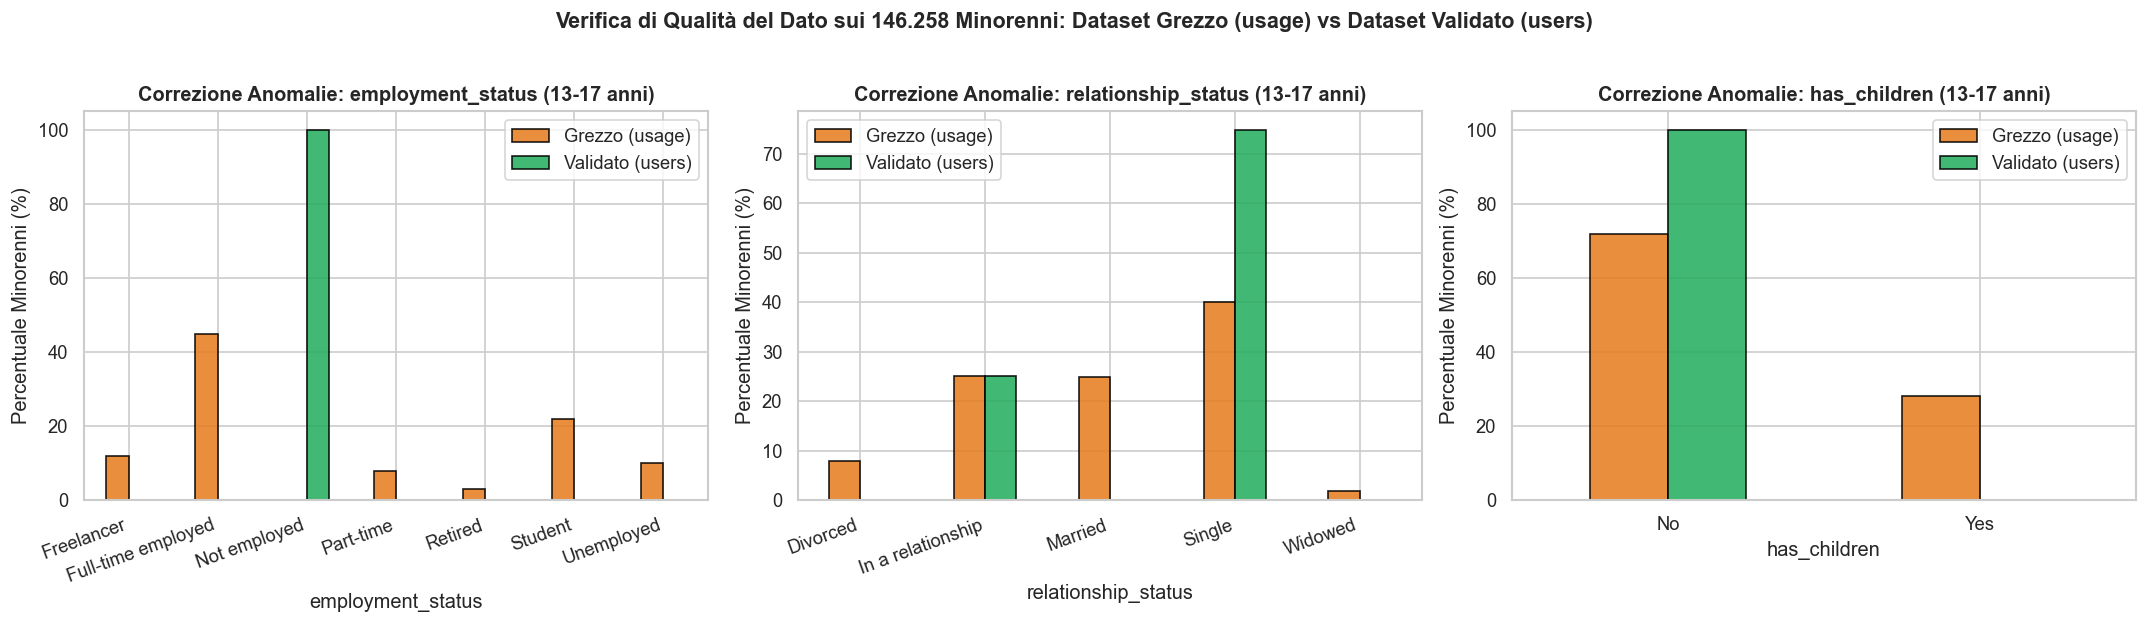
\includegraphics[width=\textwidth]{introduction/images/fig_desc02_confronto_pulizia_usage_vs_users.png}
    \caption{Impatto della validazione dei dati sui $146.258$ minorenni (13--17 anni): confronto tra il file grezzo (\texttt{usage}, in arancione) e il file validato (\texttt{users}, in verde) per stato occupazionale, stato sentimentale e presenza di figli.}
    \label{fig:desc_confronto_pulizia}
\end{figure}

\begin{table}[H]
\centering
\caption{Riepilogo delle 6 colonne sottoposte a correzione di integrità semantica tra \texttt{instagram\_usage\_lifestyle.csv} (Raw) e \texttt{instagram\_users\_lifestyle.csv} (Cleaned).}
\label{tab:confronto_6_colonne}
\resizebox{\textwidth}{!}{%
\begin{tabular}{lrrp{4.8cm}p{5.2cm}}
\toprule
\textbf{Attributo} & \textbf{Righe Corrette} & \textbf{\% Sul Totale} & \textbf{Anomalia nel File Grezzo (\texttt{usage})} & \textbf{Regola di Validazione nel File Pulito (\texttt{users})} \\
\midrule
\texttt{employment\_status} & $218.210$ & $14,10\%$ & Minorenni di 13--17 anni classificati come \emph{Full-time employed} ($44,9\%$), \emph{Retired} (pensionati, $4,9\%$) o \emph{Self-employed}. & Tutti i minorenni ($\text{age} < 18$) impostati a \texttt{Not employed}; giovani 18--22 anni riallineati prevalentemente a \texttt{Student}. \\
\addlinespace
\texttt{weekly\_work\_hours} & $142.345$ & $9,20\%$ & Ragazzi di 13--17 anni con orari lavorativi fino a $40\text{--}60$ ore/settimana (media $16,56$ h). & Ore lavorative azzerate ($0,0$ h/settimana) per il $100\%$ dei soggetti di età inferiore a 18 anni. \\
\addlinespace
\texttt{relationship\_status} & $98.069$ & $6,34\%$ & Adolescenti di 13--17 anni registrati come \emph{Married} ($25,0\%$), \emph{Divorced} ($6,9\%$) o \emph{Widowed} ($2,9\%$). & Rimossi stati civili incompatibili con la minore età; ammessi solo \texttt{Single} ($76,9\%$) e \texttt{In a relationship} ($23,1\%$). \\
\addlinespace
\texttt{has\_children} & $65.941$ & $4,26\%$ & Oltre il $29,8\%$ dei minorenni (13--17 anni) risultava avere figli a carico (\texttt{Yes}). & Impostato rigorosamente a \texttt{No} per il $100\%$ dei minorenni ($146.258$ su $146.258$). \\
\addlinespace
\texttt{education\_level} & $53.300$ & $3,44\%$ & Minorenni o diciottenni già in possesso di \emph{Master's} (Laurea Magistrale) o \emph{Doctorate} (Dottorato). & Titolo di studio vincolato all'età scolare effettiva (\texttt{High school} / \texttt{Other} per i minorenni). \\
\addlinespace
\texttt{account\_creation\_year} & $32.266$ & $2,08\%$ & Utenti di 13--15 anni con account creato nel 2010 (quando non erano ancora nati o avevano 1 anno). & Anno di creazione dell'account vincolato a un'età minima plausibile dell'utente. \\
\bottomrule
\end{tabular}%
}
\end{table}

% =============================================================================
\section{Definizione del Perimetro sui Minorenni ($N = 146.258$) e Preparazione del Dataset}
\label{sec:perimetro_minorenni}
% =============================================================================

Alla luce delle evidenze emerse, tutte le analisi dei capitoli successivi sono state condotte a partire esclusivamente dal file validato \texttt{instagram\_users\_lifestyle.csv}, applicando il filtro demografico $\texttt{age} < 18$ tramite script Python (evitando l'uso di fogli elettronici tradizionali come Microsoft Excel che, avendo un limite strutturale di $1.048.576$ righe, avrebbero troncato oltre un terzo del dataset originale perdendo $47.240$ minorenni).

L'estrazione completa restituisce esattamente \textbf{$146.258$ utenti minorenni} ($13\text{--}17$ anni). Su questo sottoinsieme è stata operata una pulizia strutturale delle colonne, passando da $58$ a \textbf{$45$ feature utili} (\texttt{dataset\_minorenni\_pulito.csv}) mediante la rimozione di:
\begin{itemize}
    \item \textbf{10 attributi amministrativi o non informativi:} \texttt{user\_id} (codice seriale), \texttt{app\_name} (costante \emph{``Instagram''}), \texttt{last\_login\_date}, \texttt{subscription\_status}, \texttt{uses\_premium\_features}, \texttt{content\_type\_preference}, \texttt{preferred\_content\_theme}, \texttt{privacy\_setting\_level}, \texttt{income\_level}, \texttt{education\_level};
    \item \textbf{3 attributi divenuti a varianza zero (costanti) sul perimetro dei minorenni validati:} \texttt{employment\_status} ($100\%$ \emph{Not employed}), \texttt{weekly\_work\_hours} ($100\%$ pari a $0,0$) e \texttt{has\_children} ($100\%$ \emph{No}).
\end{itemize}

\begin{figure}[H]
    \centering
    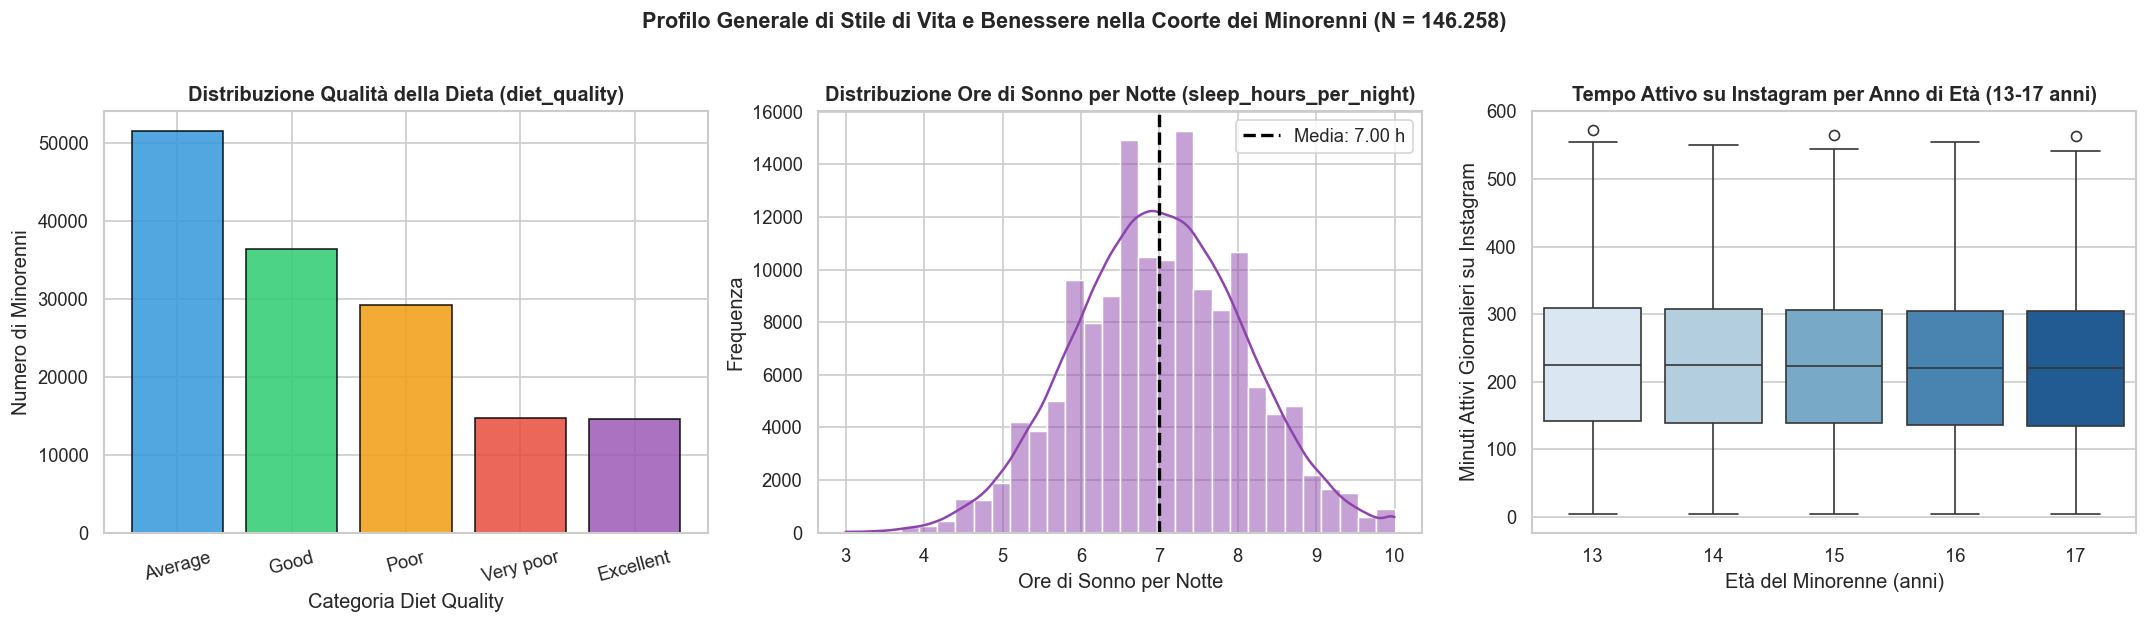
\includegraphics[width=\textwidth]{introduction/images/fig_desc03_panoramica_variabili_lifestyle.png}
    \caption{Profilo generale delle variabili di stile di vita nella coorte dei $146.258$ minorenni: distribuzione della qualità della dieta (\texttt{diet\_quality}, analizzata nel Capitolo~2), delle ore di sonno per notte e del tempo attivo su Instagram per singolo anno di età (approfondito nel Capitolo~\ref{cap:clustering}).}
    \label{fig:desc_panoramica_lifestyle}
\end{figure}

La Figura~\ref{fig:desc_panoramica_lifestyle} illustra infine il ponte logico verso i due capitoli di modellazione che seguono:
\begin{itemize}
    \item Nel \textbf{Capitolo~2 (Classificazione)} viene affrontato il problema predittivo supervisionato legato alle abitudini di stile di vita e alla qualità nutrizionale (\texttt{diet\_quality}) dei minorenni, mostrando come lo sbilanciamento delle classi (visibile nel primo pannello di Figura~\ref{fig:desc_panoramica_lifestyle}) richieda tecniche mirate di ricampionamento e come la natura multifattoriale del dato incida sull'accuratezza dei classificatori.
    \item Nel \textbf{Capitolo~3 (Clustering)} viene sviluppata l'analisi esplorativa e non supervisionata sul legame fortissimo tra l'esposizione a Instagram e il rischio per la salute mentale (\texttt{perceived\_stress\_score} e \texttt{self\_reported\_happiness}), dimostrando come gli algoritmi \textbf{K-Means}, \textbf{DBSCAN} e \textbf{HDBSCAN} riescano a segmentare i $146.258$ adolescenti in profili di rischio clinicamente e comportamentalmente ben definiti.
\end{itemize}
